% Copyright (C) Maximiliano Curia <maxy@gnuservers.com.ar>,
%               Margarita Manterola <marga@marga.com.ar>

% Esta obra está licenciada de forma dual, bajo las licencias Creative
% Commons:
%  * Atribución-Compartir Obras Derivadas Igual 2.5 Argentina
%    http://creativecommons.org/licenses/by-sa/2.5/ar/
%  * Atribución-Compartir Obras Derivadas Igual 3.0 Unported
%    http://creativecommons.org/licenses/by-sa/3.0/deed.es_AR.
%
% A su criterio, puede utilizar una u otra licencia, o las dos.
% Para ver una copia de las licencias, puede visitar los sitios
% mencionados, o enviar una carta a Creative Commons,
% 171 Second Street, Suite 300, San Francisco, California, 94105, USA.

\renewcommand{\chaptermark}[1]{\markboth{#1}{}}
\renewcommand{\thesection}{\arabic{section}}
\chapter*{Parámetros por línea de comandos}

Se le llaman parámetros de línea de comandos a todo lo que se escriba después
del nombre del programa en la invocación de un comando. Por ejemplo, hemos
dicho que para compilar se usa una línea de la forma:

\begin{verbatim} 
gcc hola.c -o hola
\end{verbatim} 

En este caso, estamos invocando al compilador \verb!gcc! para que compile
\verb!hola.c! y genere el archivo ejecutable \verb!hola!. Esto es posible,
ya que el sistema operativo le pasa al gcc los parámetros que escribió el
usuario al invocarlo, de forma que los parámetros que recibe gcc son:

\begin{codigo-c-plano}
"gcc", "hola.c", "-o", "hola"
\end{codigo-c-plano}

En nuestro código, para recibir estos parámetros se utiliza, tradicionalmente,
la \textit{firma} de la función \lstinline!main! que recibe parámetros:
  
\begin{codigo-c-plano}
int main(int argc, char *argv[]);
\end{codigo-c-plano}

En este caso recibimos en \lstinline!main! los parámetros de la invocación
del programa.  El primer parámetro será la cantidad de parámetros que se
reciben y el segundo parámetro en un vector de punteros a caracteres.

Como se vio anteriormente, cada puntero a caracteres, es la dirección de
memoria de un bloque de caracteres.

\begin{figure}[htb]
\centering
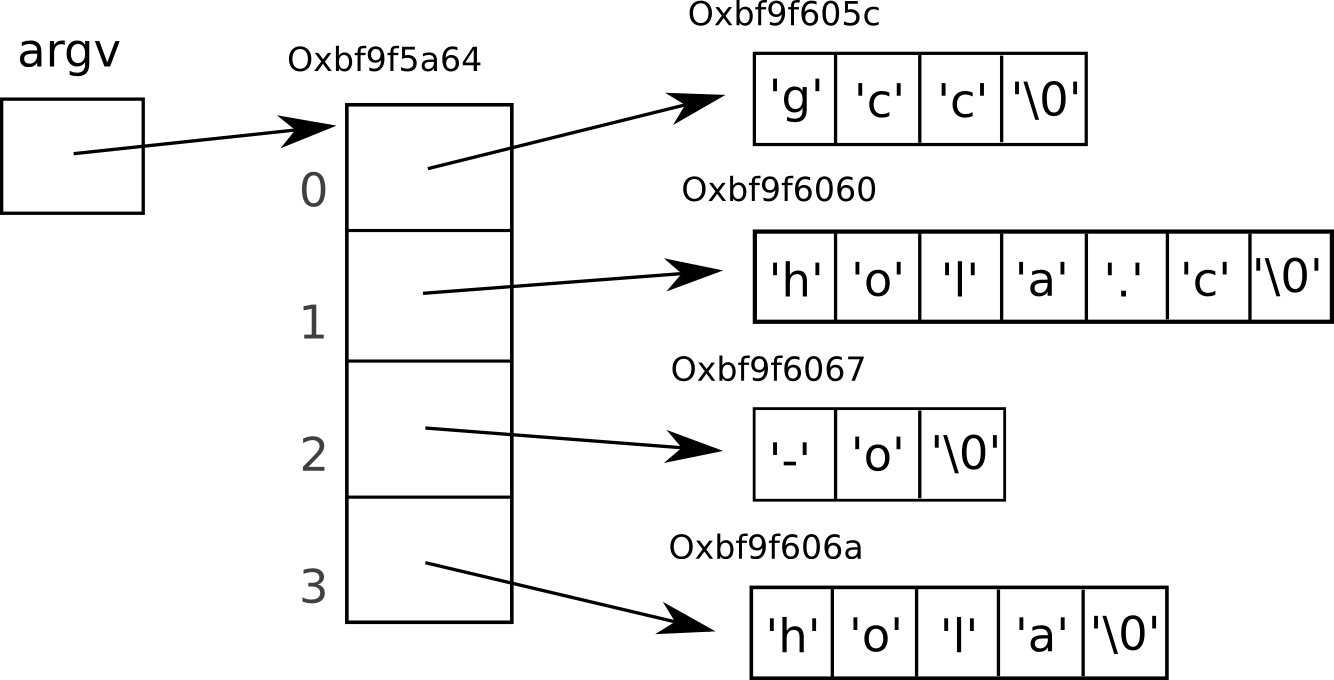
\includegraphics{imagenes/parametros}
\caption{Estructura de los parámetros recibidos por la línea de comandos
al compilar}
\end{figure}

Notar que la primera cadena apuntada por \lstinline!argv!, es el nombre del
comando que se llamó.

\section{Ejemplo de recibir parámetros por línea de comandos}

En UNIX existe un comando llamado \textbf{echo} cuya única función es imprimir todos
los parámetros que se reciben por línea de comandos. Cada parámetro se imprime
con un espacio entre parámetro y parámetro. Este sencillo programa puede
escribirse en C de la siguiente forma.

\begin{codigo-c}
#include <stdio.h>
int main(int argc, char *argv[])
{
    if (argc > 1) {
        printf("%s", argv[1]);
    }
    for (int i=2; i<argc; i++) {
        printf(" %s", argv[i]);
    }
    printf("\n");
    return 0;
}
\end{codigo-c}

En este código imprimimos todos los parámetros recibidos, omitiendo el
nombre del comando (\lstinline!argv[0]!).
Una vez compilado se lo puede invocar de la siguiente forma:
    
\begin{verbatim} 
./echo primer_parámetro  segundo_parámetro   etc
\end{verbatim} 

Y sin importar la cantidad de espacios entre un parámetro y otro el resultado
será: 

\begin{verbatim} 
primer_parámetro segundo_parámetro etc
\end{verbatim}

